
An informal proof for the optimized schedule factory's soundness and correctness follows. Suppose an HJ program data races on Thread A and B. In order for the two threads to data race, the threads will need to be alive at one point of execution. \figref{fig:proof} shows a simplified execution process for JPF using the optimized scheduler to find a data race with \texttt{ChoiceGenerators} with creation of new threads and shared field accesses.

First, there is a \texttt{ChoiceGenerator} that has these two threads before the shared field is accessed (such as the creation of thread B). Thread A is executed first (i). The shared field is accessed by A, and JPF stores this access using global search object IDs. However, on this execution, JPF is unaware that Thread B accesses the shared field, and continues running. Thread A terminates, and JPF switches to a different thread, though a new \texttt{ChoiceGenerator} is not created. Thread B executes, and runs till B accesses the shared field. JPF stores this access using the global search object ID and finds that A also accesses it. However, since Thread A no longer is alive, a \texttt{ChoiceGenerator} is not created, and B continues to run till it terminates.

At the end of the execution, JPF back tracks to the last \texttt{ChoiceGenerator} (ii) and picks to execute Thread B. JPF executes B until B accesses the shared field. The global search object ID once again determines that Thread A also accesses the field. However, since Thread A is alive, a \texttt{ChoiceGenerator} is created. Thread B continues (iii) execution until termination, and Thread A then executes. As before (i), Thread A executes till it reaches the shared field, but finds that Thread B is no longer alive, so no \texttt{ChoiceGenerator} is created. Thread A terminates, and JPF backtracks to the last \texttt{ChoiceGenerator} and executes a different thread (iv). Thread A is selected and executed. When Thread A reaches the shared field access, JPF checks its global search object ID, finds that Thread B is still alive, and inserts another \texttt{ChoiceGenerator}.

At this point, JPF's \texttt{PreciseRaceDetector} searches at the \texttt{ChoiceGenerator} (and has been doing at all \texttt{ChoiceGenerators} thus far) for two threads that have a shared field access on the same field. If there are, which Thread A and B are, then \texttt{PreciseRaceDetector} makes an additional check for at least one being a write in order to report a data race. Since Thread A and B do, JPF with the optimized scheduler reports a data race.
\begin{figure}[t]
\begin{center}
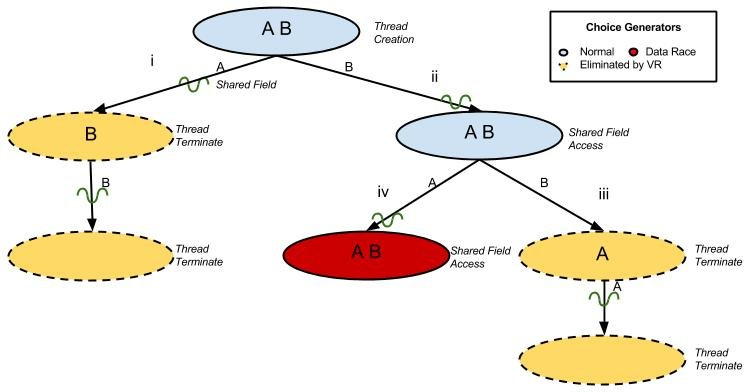
\includegraphics[width=3.25in]{../figs/InformalProofDiagram}
\end{center}
\vspace{-10pt}
\caption{A JPF search illustrating the scheduler.}
\label{fig:proof}
\end{figure}
